\documentclass{beamer}

\usepackage{helvet}
\usepackage{hyperref, graphicx}
\usepackage{amsthm, amsfonts}
\usepackage{etoolbox}
%\usepackage{multicol}
%\usepackage{tikz}
\usepackage{caption}
\usepackage{ulem}

%% Define the layout of slides, numbering, and color theme
%% Also, make links in TOC appear at start of each section 
\usetheme[progressbar=frametitle, numbering=none]{metropolis}
\usecolortheme[snowy]{owl}
\setbeamertemplate{navigation symbols}{}
\AtBeginSection[ ]
{
\begin{frame}{Outline}
    \tableofcontents[currentsection]
\end{frame}
}

%% Default fixed font does not support bold face
\DeclareFixedFont{\ttb}{T1}{txtt}{bx}{n}{11} % for bold
\DeclareFixedFont{\ttm}{T1}{txtt}{m}{n}{12}  % for normal - use in headings

%% Custom colors
\usepackage{color}
\definecolor{TUGray}{RGB}{101,101,137}
\definecolor{TUBlack}{RGB}{0,0,10}
\definecolor{mygreen}{RGB}{45,111,63}
\definecolor{keywords}{RGB}{205,114,0}
\definecolor{comments}{RGB}{181,51,139}
\definecolor{strings}{RGB}{58,144,81}
\definecolor{numeric}{RGB}{66,110,176}
\definecolor{linos}{rgb}{0.4,0.4,0.4}
\definecolor{links}{rgb}{0,0.4,0.75}

\definecolor{bggray}{RGB}{232, 233, 235}

\setbeamercolor{alerted text}{fg=mygreen}
\setbeamercolor{normal text}{fg=TUBlack}\usebeamercolor*{normal text}

\setbeamercolor{codecol}{fg=TUGray!25!black,bg=bggray}

%% Coloring of links
\hypersetup{colorlinks, linkcolor=links, urlcolor=links}

%% Custom multi-line commenting out
\newcommand{\comment}[1]{}

%% Fonts
\usepackage[T1]{fontenc}
\usepackage[sfdefault,scaled=.85]{FiraSans}
\usepackage{newtxsf}

%% Package for displaying lines of code, or pseudocode
\usepackage{listings}

\newtoggle{InString}{}% Keep track of if we are within a string
\togglefalse{InString}% Assume not initally in string

%% Some line parsing in listings code blocks, to perform highlighting (digits,keywords, comments, etc)
\newcommand\digitstyle{\color{numeric}}
\makeatletter
\newcommand{\ProcessDigit}[1]
{%
  \ifnum\lst@mode=\lst@Pmode\relax%
   {\digitstyle #1}%
  \else
    #1%
  \fi
}
\makeatother

\lstset{literate=%
    {0}{{{\ProcessDigit{0}}}}1
    {1}{{{\ProcessDigit{1}}}}1
    {2}{{{\ProcessDigit{2}}}}1
    {3}{{{\ProcessDigit{3}}}}1
    {4}{{{\ProcessDigit{4}}}}1
    {5}{{{\ProcessDigit{5}}}}1
    {6}{{{\ProcessDigit{6}}}}1
    {7}{{{\ProcessDigit{7}}}}1
    {8}{{{\ProcessDigit{8}}}}1
    {9}{{{\ProcessDigit{9}}}}1
	{<=}{{\(\leq\)}}1
	{>=}{{\(\geq\)}}1,
	% morestring=[b]",
    % morestring=[b]',
    % morecomment=[l]{//},
}

%% Defining keywords and comment formatting for a pseudocode block
\lstdefinelanguage{Pseudo}{
    morekeywords={return, while, if, for, input},
    morecomment=[l]{\#},
}

%% Pseudocode style
\newcommand\pseudostyle{\lstset{
language=Pseudo,
basicstyle=\fontfamily{ccr}\scriptsize,
commentstyle=\it\scriptsize\color{linos},
keywordstyle=\it\bfseries\scriptsize,
mathescape=true,
literate=
    {=}{$\leftarrow{}$}{1}
    {==}{$={}$}{1}
    {<=}{{\(\leq\)}}1
	{>=}{{\(\geq\)}}1,
xleftmargin=18pt,
xrightmargin=4pt,
aboveskip=12pt,
belowskip=0pt,
frame=tB,
keepspaces=true
}}

%% Python style
\newcommand\pythonstyle{\lstset{
language=Python,
basicstyle=\ttfamily\tiny,
numbers=left,
numberstyle=\tiny\color{linos},
morekeywords={self, np},              % Add keywords here
keywordstyle=\tiny\color{keywords},
commentstyle=\it\tiny\color{comments},    % Custom highlighting style
stringstyle=\tiny\color{strings},
xleftmargin=18pt,
xrightmargin=4pt,
aboveskip=0pt,
belowskip=0pt,
escapeinside={(*@}{@*)},
frame=l,                         % Any extra options here
showstringspaces=false,
keepspaces=true
}}

%% Pseudocode environment
\lstnewenvironment{pseudo}[1][]
{
    \pseudostyle
    \lstset{
        #1
    }
}
{}

%% Python environment 
\lstnewenvironment{python}[1][]
{
	\pythonstyle
	\lstset{
	#1
	}
}
{}

%% wrap the Python environment
\newenvironment{codeblock}
    {\hfill\begin{beamerboxesrounded}[lower=codecol, width=0.8\textwidth]
    \medskip

    }
    { 
    \end{beamerboxesrounded}\hfill
    }

%% A couple of block enviroments to make statement stand out
\theoremstyle{example}
\newtheorem{question}{Question}

%% Some shortcut macros for computer-type font
\newcommand{\ct}[1]{\lstinline[language=Python]!#1!}
\newcommand{\st}[1]{\lstinline[language=Python,basicstyle=\ttfamily,stringstyle=\small\color{strings}]!#1!}
\newcommand{\ttt}[1]{{\small\texttt{#1}}}
\newcommand{\lsitem}[2]{\ttt{{#1}[}\ct{#2}\ttt{]}}
\newcommand{\bb}[1]{\mathbb{#1}}
\newcommand{\cl}[1]{\mathcal{#1}}

%% Header information
\author{Chris Cornwell}
\date{Aug 26, 2025}
\title{Overview of Machine Learning \newline 
    \footnotesize{with focus on Supervised Learning}}

%% Start of slides
\begin{document}

\begin{frame}
\titlepage
\end{frame}

\begin{frame}
\frametitle{Outline}
\tableofcontents
\end{frame}

\section{Machine Learning}

%% Broad discussion of machine learning
%%%%
\begin{frame}
\frametitle{What is Machine Learning?}
    \begin{itemize}
        \item Concerned with designing, understanding algorithms which allow computer program to ``learn.''
        \pause
        \item Not as new as it seems, but rapid growth in last 2 decades. 
        \begin{itemize}
            \item field of study since 1950's; 
            \item related to much older statistical modeling.
        \end{itemize}
        \pause
        \item Can be single ML model performing task (e.g., finding person in an image, speech-to-text, sentiment analysis)
        \pause
        \item Or, many separate models combined together $\leftarrow$ what makes AI work (e.g., self-driving cars, LLM's or chatbots).
    \end{itemize}
\end{frame}

%%%%
\begin{frame}
\frametitle{What is Machine Learning?}
    % Mitchell '98 ``Well posed learning problem'' - Mitchell is (old) researcher in machine learning, prof at Carnegie Melon
    \textit{Very} general, academic definition by Tom Mitchell:\newline 
    \begin{quote}
        A ``computer program'' is said to \textbf{learn} from experience $E$, with respect to some task $T$ and performance measure $M$ if: its performance on $T$, as measured by $M$, improves with experience $E$.
    \end{quote}
    \vspace*{-12pt}
    \pause
    \begin{itemize}
        \item Often, the experience $E$ is called ``training'' (updates to how program runs); based on observed data.
        \pause
        \item ``computer program,'' for us ``learning algorithm'', determines a function that produces output from given input (the data). After training, the resulting input-output function represents achieving the task $T$. 
        \pause
        \item In class, we will discuss algorithms made for \textit{regression} tasks, and others for \textit{classification} tasks, that fit this paradigm.
        \pause 
        \item Performance measure $M$: for us, called a \textit{cost function} or \textit{loss function}.
    \end{itemize}

\end{frame}

%%%%
\begin{frame}
\frametitle{Two general categories in machine learning}

\textbf{Supervised learning:} algorithm uses sample (input) data that have output ``labels.'' Goal: determine a \emph{good} underlying function from sample data.
\pause
    \begin{itemize}
        \item Housing price prediction
        \pause
        \item Whether emails are junk or not.
        \pause
        \item Detect space debris, or trash on ocean surface.
        %\item Auto-completion of typed sentence.
    \end{itemize}
\pause
\textbf{Unsupervised learning:} algorithm uses sample data, but it is unlabeled. Goal: discover something (a pattern, grouping, or some insight) about the data based on its coordinates (features).
\pause
    \begin{itemize}
        \item Market segmentation.
        \pause
        \item News feed (grouping similar news articles).
        \pause
        \item Separate audio sources in a mixed signal.
    \end{itemize}

\end{frame}

\section{Supervised learning}

%%%%
\begin{frame}
\frametitle{The goal of Supervised learning}
In Section 1.2, the textbook uses the term ``Predictive learning'' to mean same as Supervised learning. 
\begin{itemize}
    \item (Supervised $\iff$ labels) 
    \item The labeled sample data is called \textbf{training data}. The goal is to ``learn'' a function from the training data that will do well labeling new data, not seen during learning process. 
    \item ``Doing well'' is measured by a loss function ($M$ from Mitchell's description). 
    \item \invisible<1>{The learning algorithm starts with \emph{some} function; it doesn't do labeling well, but the algorithm uses the loss function to alter that function to something better. ($\leftarrow$ ``learning'')}
\end{itemize}
\end{frame}

%%%%
\begin{frame}[standout]
    Example Images
\end{frame}

%%%%
\begin{frame}
\frametitle{Example 1 - Supervised learning, Section 1.1 of textbook}
\textbf{Cat or Dog?}

\begin{figure}
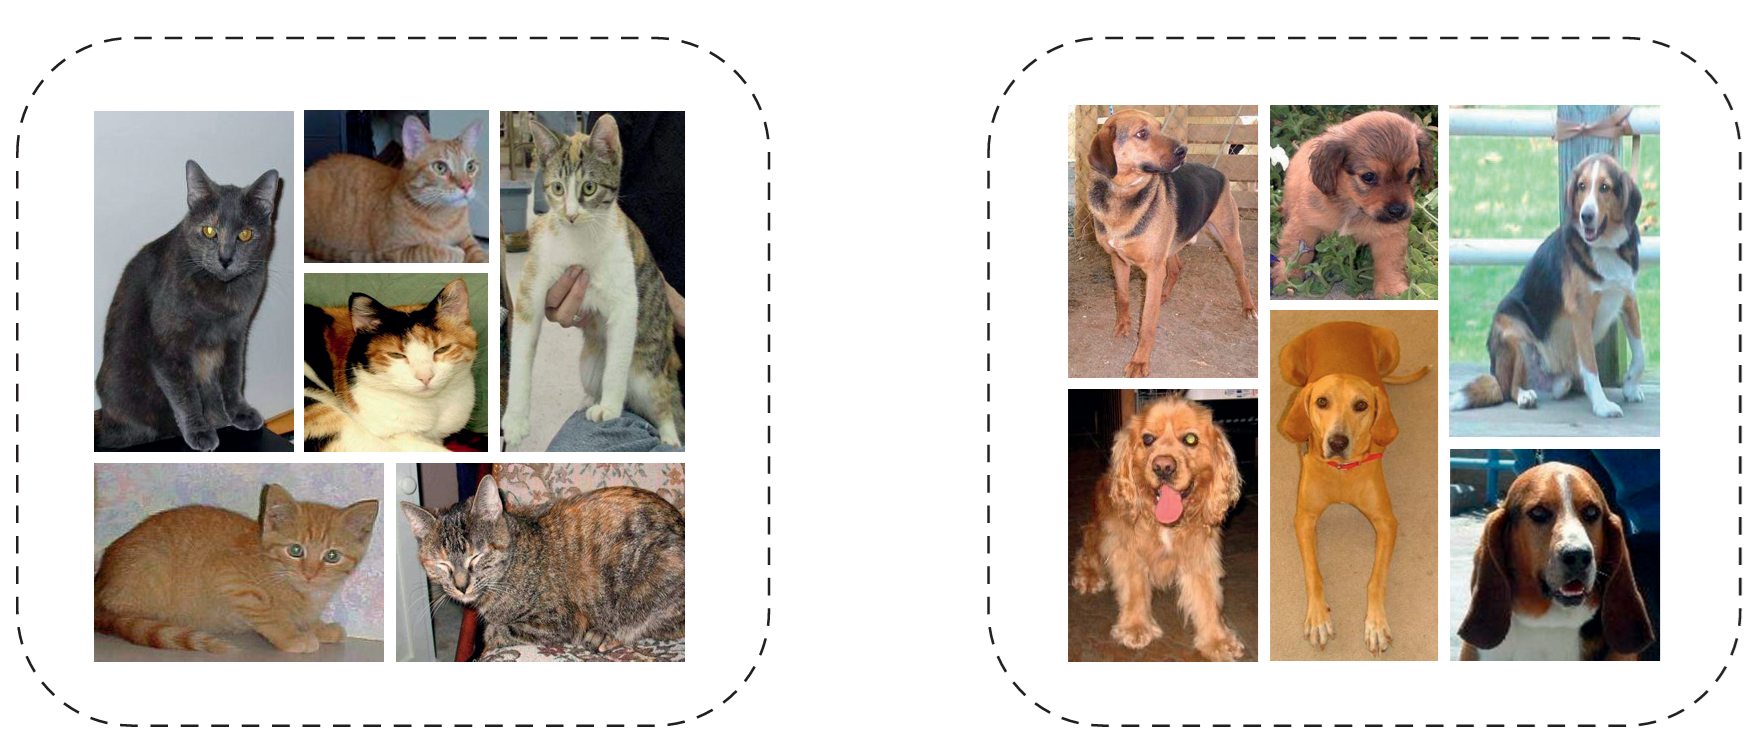
\includegraphics[width=0.45\textwidth]{../../Images/Fig1-1.png}
\caption*{Figure 1.1 from textbook}
\end{figure}

\begin{itemize}
    \item Training data. The images, each with label \st{'cat'} or \st{'dog'}.
    \item Computer sees each image, pixels in 2D array with RGB value (a vector in $\bb R^3$) at each pixel.
    \item \textbf{Designing features.} ``Cartoon image'' of ML model's function: computes $N$ \textbf{features} from each image $\leadsto$ vectors (points) in $\bb R^N$ $\leadsto$ points with one label separated from those with other label (by graph of linear function).
\end{itemize}
\end{frame}

%%%%
\begin{frame}
    \frametitle{Designing features, to easily separate data}
    Compute $N$ \textbf{features} from each image $\leadsto$ vectors (points) in $\bb R^N$ $\leadsto$ points with one label separated from those with other label (by graph of linear function).

    \begin{figure}
        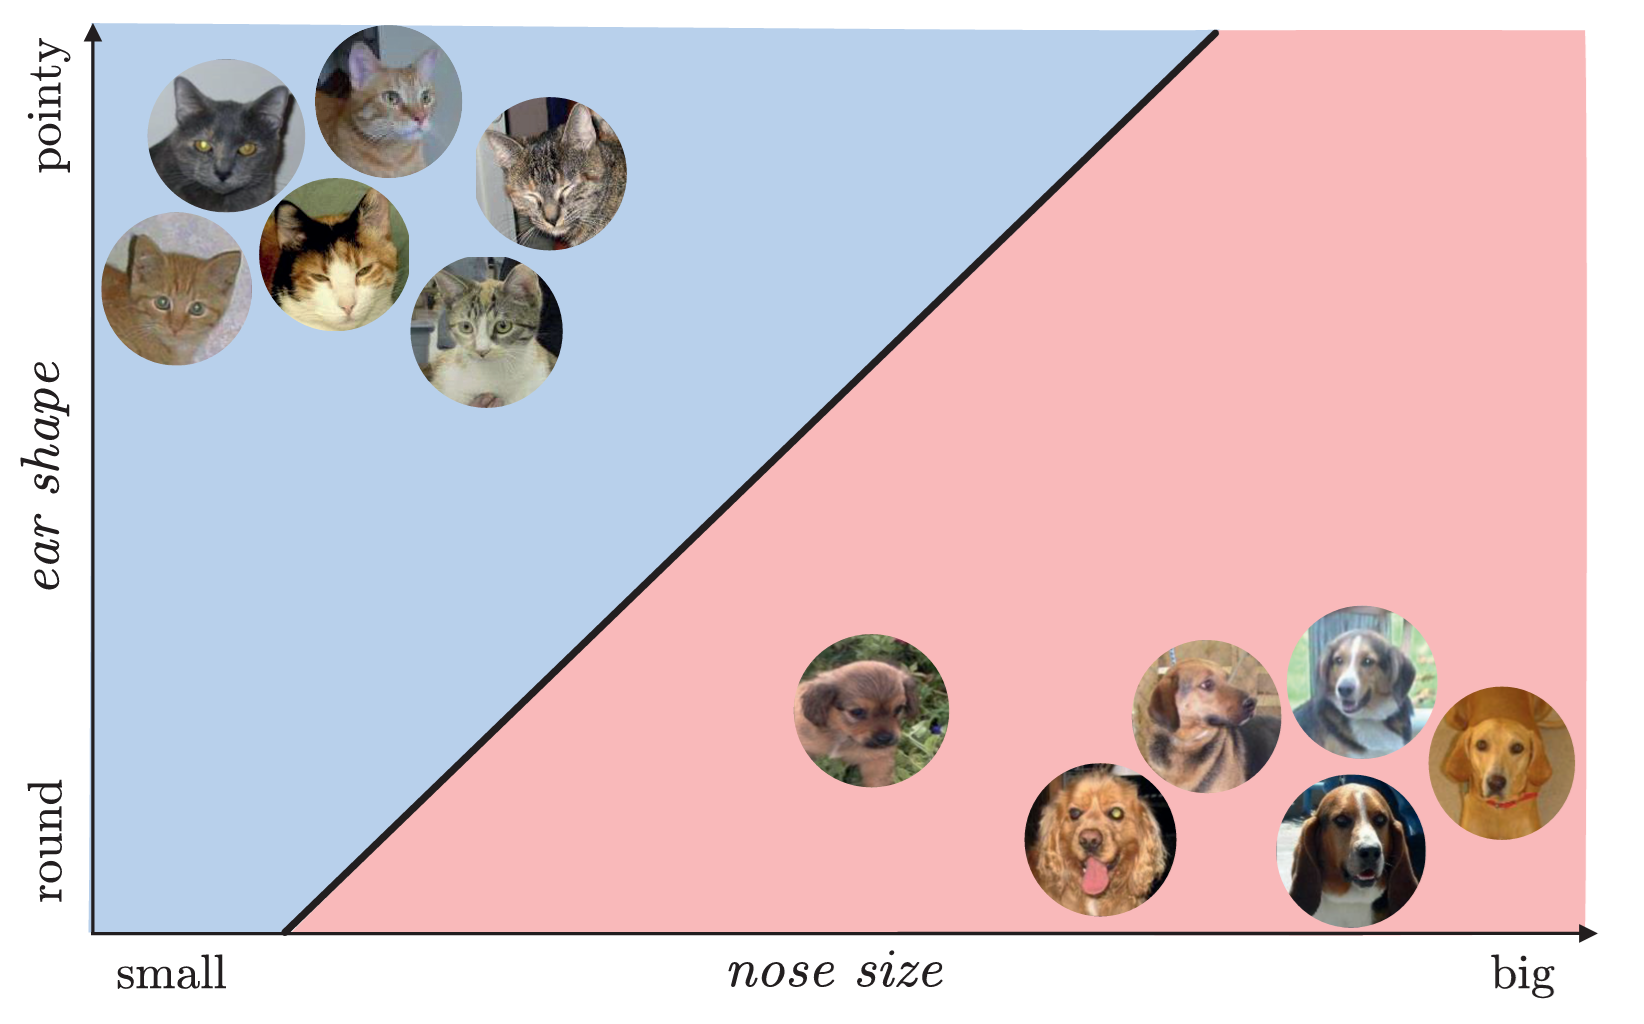
\includegraphics[width=0.8\textwidth]{../../Images/Fig1-3.png}
    \caption*{Figure 1.3 from textbook}
    \end{figure}
\end{frame}

%%%%
\begin{frame}
\frametitle{Example 2 - Supervised learning, Section 1.2 of textbook}
\textbf{Predict share price}

\begin{figure}
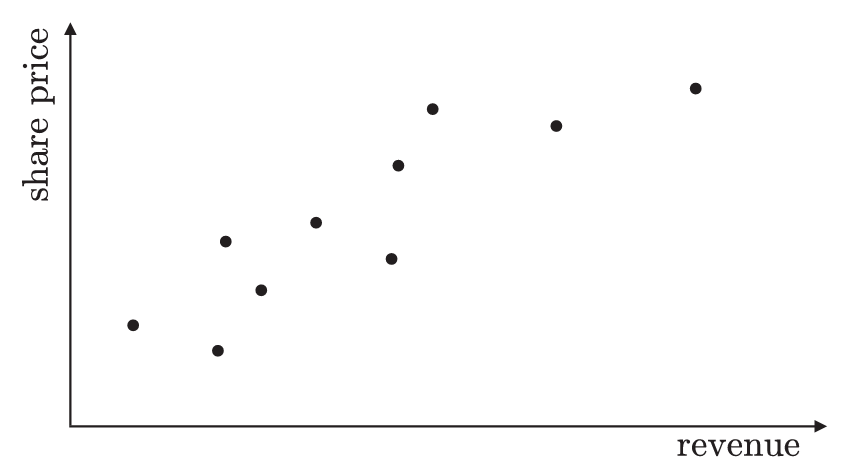
\includegraphics[width=0.4\textwidth]{../../Images/Fig1-7a.png}
\caption*{Figure 1.7, upper-left from textbook}
\end{figure}

\begin{itemize}
    \item From training data, pick one feature: revenue. Label: the share price.
    \item Each revenue, a number in $\bb R$. One ``independent variable,'' call it $x$.
    \item \textbf{Designing features.} Here, have used a feature already at hand. Not always best idea when there are multiple independent variables (we'll see examples later, where you design features).
\end{itemize}
\end{frame}

%%%%
\begin{frame}
    \frametitle{Example 2 - Predict response variable, share price}
    Revenue value: $x$.  Find a function $f(x) = \hat{m}x + \hat{b}$, so that if $y$ is share price for $x$ and we set $\hat{y} = f(x)$ then $y$ and $\hat{y}$ are close, on average. (Linear Regression)

    \begin{figure}
        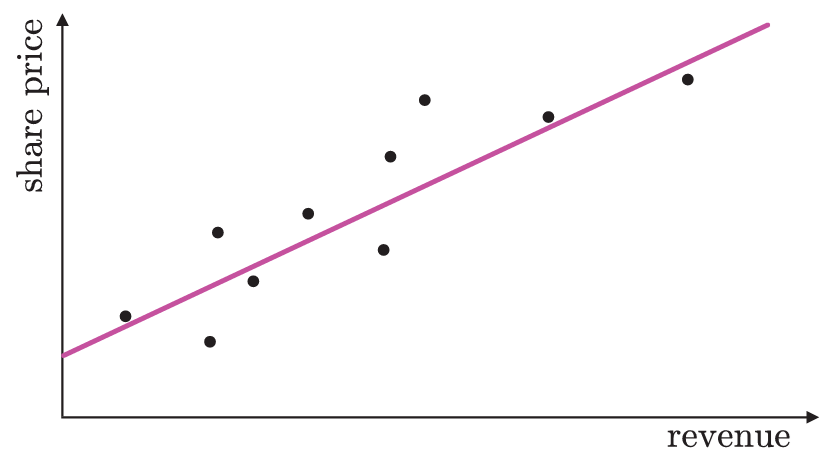
\includegraphics[width=0.8\textwidth]{../../Images/Fig1-7b.png}
    \caption*{Figure 1.7, upper-right from textbook}
    \end{figure}
\end{frame}

%%%%
\begin{frame}
\frametitle{Supervised learning, very generally}
Have an ``input space'' (often is $\mathbb R^{N}$, for some $N$, or subset of it\footnote{The domain (input space) \textit{could} be some different space.}).  Have an output space, or label space, $Y$. ($Y$ is a finite list of labels for classification; it is $\bb R$ or an interval in $\bb R$ for regression.) 

\pause
\begin{itemize}
    \item Given a sample $\mathcal S = \{({\bf x}_i, y_i)\}_{i=1}^P$, with ${\bf x}_i\in\mathbb R^N$ and $y_i\in Y$, drawn from an (unknown) joint probability distribution $\rho_{X,Y}:\mathbb R^{N}\times Y \to [0, \infty)$. 
    \pause
    \item Goal: to learn, from $\mathcal S$, a function $f^*:\mathbb R^N\to Y$ that ``fits'' (\textit{approximates well}) the distribution $\rho_{X,Y}$. 
    \pause
    \item Might not be possible for points on graph of $f^*$ to be typically ``close'' to samples from $\rho_{X,Y}$. However, for an ${\bf x}\in\mathbb R^N$, the corresponding $f^*(\bf x)$ should be near expected value of $y$, given ${\bf x}$.
\end{itemize}

\end{frame}

%%%%
\begin{frame}
\frametitle{Achieving the general goal}
Most often, we choose a \textit{parameterized class} of functions\footnote{Sometimes called a \textit{hypothesis class}.}, and we get $f^*$ from that class. 
\pause
\begin{itemize}
    \item Have space of parameters $\Omega$; an $\omega\in\Omega$ determines a function $f_{\omega}:\mathbb R^N \to Y$. The parameterized class is the set of all such $f_\omega$. % Model selection
    \pause
    \item Change parameters to find a function that fits well.
\end{itemize}

\pause
How to change parameters?  Select a performance measure: \textbf{(empirical) loss function} $\mathcal L_{\mathcal S}:\Omega \to \mathbb R$. %In the empirical loss function, we use $\mathcal S$ in its definition.
\begin{itemize}
    \pause
    \item Want to make value of $\mathcal L_{\mathcal S}$ small; use the function itself to do this.
    \pause
    \item Ideally, converge to some $\omega^*$, a minimizer of $\mathcal L_{\mathcal S}$, and set $f^* = f_{\omega^*}$.
\end{itemize}

\end{frame}

\comment{
%%%%
\begin{frame}
    \frametitle{For linear regression}
    Have sample data $\mathcal S$, with data points $x_i$ in $\mathbb R$ (so, $d=1$). The parameter space $\Omega = \mathbb R^2 = \{(m,b)\ |\ m\in\mathbb R, b\in\mathbb R\}$. For each $\omega = (m,b)$, we have
        \[f_{\omega}(x) = mx + b.\]
    \pause
    Loss function: the MSE. That is, set 
        \[\mathcal L_{\mathcal S}(m,b) = \frac1{n}\sum_{i=1}^n (mx_i + b - y_i)^2.\]
\end{frame}

\section{First look at Gradient Descent}

%%%%
\begin{frame}
\frametitle{Gradient descent with simple linear regression}
For $\omega = (m, b)$, have $f_{\omega}(x) = mx + b$. Given sample data $\mathcal S=\{({\bf x}_i, y_i)\}_{i=1}^n$, note that the empirical loss function $\mathcal L_{\mathcal S}$ is a function of $m$ and $b$ (while $\mathcal S$ is \textit{used} in its definition, the points ${\bf x}_i$ are not inputs to $\mathcal L_{\mathcal S}$).
\pause 

Recall the definition $\mathcal L_{\mathcal S}(m,b) = \frac1{n}\sum_{i=1}^n (mx_i + b - y_i)^2$.
\begin{itemize}
    \item The \textbf{gradient} of $\mathcal L_{\mathcal S}$ is the vector of partial derivatives: $\nabla\mathcal L_{\mathcal S} = \left( \frac{d}{dm}\mathcal L_{\mathcal S}, \frac{d}{db}\mathcal L_{\mathcal S} \right)$.
    \pause
    \item Get partial derivatives using the Chain rule: 
            \[\frac{d}{dm}\mathcal L_{\mathcal S} = \frac{2}{n}\sum_{i=1}^n(mx_i + b - y_i)x_i;\]
        and 
            \[\frac{d}{db}\mathcal L_{\mathcal S} = \frac{2}{n}\sum_{i=1}^n(mx_i + b - y_i).\]
\end{itemize}

\end{frame}

%%%%
\begin{frame}
    \frametitle{Aside: Recovering the normal equations}
    By utilizing the fact that a minimum of $\mathcal L_{\mathcal S}$ only occurs when $\frac{d}{dm}\mathcal L_{\mathcal S} = 0$ and $\frac{d}{db}\mathcal L_{\mathcal S} = 0$,
    we can recover the normal equations.
    
    \pause
    To simplify it (and still be able to generalize), say that we have $n=3$ (in other words, $\mathcal S$ has just three points). Then, setting ${\bf x} = (x_1,x_2,x_3)$ and ${\bf y} = (y_1,y_2,y_3)$, and $\bar{x}$ equal to the average of $x_1,x_2,x_3$,
    \pause
    {\small
        \begin{align*}
            \frac{d}{dm}\mathcal L_{\mathcal S}     &= \frac{2}{3}\left((mx_1^2 + bx_1 - x_1y_1) + (mx_2^2 + bx_2 - x_2y_2) + (mx_3^2 + bx_3 - x_3y_3) \right) \\ 
                                                    &= \frac{2}{3}\left(m(x_1^2+x_2^2+x_3^2) + b(x_1+x_2+x_3) - (x_1y_1+x_2y_2+x_3y_3) \right) \\ 
                                                    &= \frac{2}{3}\left(m{\bf x}\cdot{\bf x} + b(3\bar{x}) - {\bf x}\cdot{\bf y}\right).
        \end{align*}
    }
    
    \pause
    And so, setting $\frac{d}{dm}\mathcal L_{\mathcal S} = 0$ amounts to the equation $m({\bf x}\cdot{\bf x}) + b(3\bar{x}) = {\bf x}\cdot{\bf y}$. 

    \pause
    A similar computation will show that setting $\frac{d}{db}\mathcal L_{\mathcal S} = 0$ will give the equation $m(3\bar{x}) + b(3) = 3\bar{y}$. (With $\bar{y}$ being the average of $y_1,y_2,y_3$). 
\end{frame}

%%%%
\begin{frame}
    \frametitle{Aside: Recovering the normal equations}
    The computation above generalizes to imply that $\nabla\mathcal L_{\mathcal S} = (\frac{d}{dm}\mathcal L_{\mathcal S}, \frac{d}{db}\mathcal L_{\mathcal S}) = (0,0)$ requires the equations 
        \begin{align*}
            m({\bf x}\cdot{\bf x}) + b(n\bar{x})    &= {\bf x}\cdot{\bf y} \\ 
            m(n\bar{x}) + b(n)                      &= n\bar{y}.
        \end{align*}
    
    \pause 
    If you recall the entries in $A^TA$ and $A^T{\bf y}$ (where $A$ is the matrix built in the simple linear regression procedure), these are precisely the normal equations.

    Solving for $m$ and $b$ gives us $m = \frac{{\bf x}\cdot{\bf y} - n\bar{x}\bar{y}}{{\bf x}\cdot{\bf x} - n\bar{x}^2} = \frac{\sum_{i=1}^n(x_i - \bar{x})(y_i - \bar{y})}{\sum_{i=1}^n(x_i - \bar{x})^2}$, and $b = \bar{y} - m\bar{x}$.

    \pause 
    \begin{itemize}
        \item We are able to nicely represent the minimizer of $\mathcal L_{\mathcal S}$ precisely because of the linear nature of the class of functions $f_{\omega}(x) = mx+b$.
    \end{itemize}
\end{frame}

%%%%
\begin{frame}
    \frametitle{Returning to Gradient Descent}
    In anticipation that, in other settings, we not be able to nicely represent a minimizer of $\mathcal L_{\mathcal S}$, we consider another optimization approach. 

    \pause
    \begin{itemize}
        \item Say that the (current) value of $\omega$ is $(m_0, b_0)$. Then, recalling from Calculus III, the direction of \textit{steepest descent}, that will produce the most rapid decrease in the value of $\mathcal L_{\mathcal S}$, is the direction of $-\nabla\mathcal L_{\mathcal S}(m_0,b_0)$.
        \item This indicates that we might be able to get closer to a minimizer by subtracting the gradient from $(m_0,b_0)$ or, to make our step ``small'' perhaps, subtracting a small multiple of the gradient.
    \end{itemize}

    \pause
    \textbf{Gradient descent:} Choosing a constant $\eta > 0$ and given some current value of $\omega_i = (m_i,b_i)$, we attempt to get closer to the minimizer, $\omega^*$, of the loss function by the update 
        \[\omega_{i+1} = \omega_i - \eta\ast\nabla\mathcal L_{\mathcal S}(m_i,b_i).\]
    The constant $\eta$ is called the \textbf{learning rate}.
\end{frame}

%%%%
\begin{frame}
    \frametitle{Sources}
    The content of these slides has been combined from two references. 

    \begin{enumerate}
        \item Notes taken from Machine Learning course, taught by Andrew Ng, Stanford U.
        \item Notes from a lecture series on Deep Learning at Harvard, taught by Eli Grigsby.
    \end{enumerate}

    \vfill
\end{frame}
}

{\setbeamercolor{palette primary}{fg=mygreen, bg=bggray}
\begin{frame}[standout]
    Questions?
\end{frame}
}
\end{document}